\section{Results and Discussion}

\subsection{Reward Models}
Reward model classification results are shown in Table~\ref{tab:reward_model}. The F1 score is calculated as binary, and the ROC curve is based on the probability (softmax across two samples on the positive logit) of the wide-spectrum aesthetics sample being correctly selected. We included GPT-5 Chat as an external baseline to validate the LLM-as-judge choices (when GPT-5-Chat selected a tie, we assigned it to the original image). Reward models perform very poorly when tasked with selecting the better image under the \textbf{wide-spectrum aesthetics prompt}, sometimes worse than random guessing (HPSv3), and most are worse than their CLIP and BLIP base models. The unaligned BLIP and CLIP can correctly identify the better-fitting image, indicating that complex prompt understanding is not the underlying issue but rather biased alignment. These models do what they claimed: find ``aesthetically pleasing'' images; our point is that this task itself is problematic, and the better the model performs on it, the more troublesome it is.

Given our sample size (300), we ran a Wilcoxon signed-rank test between each aligned model and its base model on the HPSv3 and HPSv2 score $r(I_a, p_o)$ and $\sum_{d\in D}J(I_a,d)$, plus McNemar's test on the success counts, with an alternative hypothesis that the aligned model has a higher score or lower success rate (Table~\ref{tab:align_p}). Most p-values are below $1\times10^{-5}$, suggesting that aligning image generation toward generalized aesthetic goals conflicts with faithful instruction following, especially for wide-spectrum aesthetics prompts.


\subsection{Image Generation Models}
Image generation results are in Table~\ref{tab:gen}. Within each family, the preference-aligned model generally performs the worst on wide-spectrum aesthetics prompt following. Playground shows a larger $\Delta$ than SDXL, likely due to SDXL's poor and Playground's high original quality. Instruction alignment (SD3.5M-GenEval) gives a slight but weak benefit. Flux Krea, though preference-aligned, performs best in the Flux family, likely because it originates from an unaligned version (flux-dev-raw) and was not heavily aligned, or because its non-generalized alignment preserved some flexibility. Base models can do reasonably well on anti-aesthetics generations despite the more complex prompts, showing this is alignment-induced bias rather than an instruction-following failure.

The success rate indicates how often the LLM selects $I_a$ as better following $p_a$ than $I_o$. Even small advantages count as success. The DanceFlux result is notably poor: about 64\% of the time, $I_a$ performs the same or worse in wide-spectrum aesthetics compared to $I_o$.


\begin{table*}[t]
 \centering

 \caption{The results for each model. $\Delta$HPSv2, $\Delta$HPSv3, and $\Delta$ImgRewd (ImageReward) are all calculated as $r(I_a, p_o) - r(I_o, p_o)$. The lower the values, the greater the difference between the traditional quality of the original image and the wide-spectrum aesthetics image. HPSv3 AA (HPSv3 after alignment) shows the HPSv3 score of $r(I_a, p_o)$. $\Delta J$ and $J$ AA ($J$ after alignment) denote $\sum_{d\in D} J(I_a, d) - J(I_o, d)$ and $J(I_a, d)$, respectively, where $D$ is the selected set of dimensions. Success is the rate at which the LLM selects $I_a$ as the image that better describes $p_a$. }
  \scalebox{0.86}{
 \begin{tabular}{lrrrrrrl}
 \toprule
 & $\Delta$HPSv2 ($\downarrow$) & $\Delta$HPSv3 ($\downarrow$) & HPSv3 AA ($\downarrow$) & $\Delta$ImgRewd ($\downarrow$) & $\Delta J$ ($\downarrow$) & $J$ AA ($\downarrow$) & BLIP ($\uparrow$) \\
 \midrule
 Flux Dev \cite{noauthor_black-forest-labsflux1-dev_2025}& -0.035 & -3.165 & 9.070 & -0.319 & -1.092 & 8.944 & 0.893 \\
 DanceFlux \cite{xue_dancegrpo_2025}& -0.018 & -1.105 & 12.782 & -0.201 & -0.672 & 10.473 & 0.813 \\
 PrefFlux \cite{wang_pref-grpo_2025} & -0.032 & -2.771 & 10.211 & -0.278 & -1.027 & 9.343 & 0.917 \\
 Flux Krea \cite{noauthor_releasing_2025}& \textbf{-0.041} & \textbf{-4.372} & \textbf{7.705} & \textbf{-0.425} & \textbf{-1.296} & \textbf{8.774} & 0.950 \\
 \hline
 SDXL \cite{podell_sdxl_2023}& -0.034 & -4.041 & \textbf{4.439} & -0.482 & -1.136 & \textbf{8.575} & 0.915 \\
 Playground \cite{li_playground_2024} & \textbf{-0.044} & \textbf{-4.170} & 7.133 & \textbf{-0.719} & \textbf{-1.204} & 9.174 & 0.912 \\
 \hline
 SD3.5M & -0.027 & -5.175 & 6.537 & -0.409 & -1.307 & 8.334 & 0.938 \\
 SD3.5M-GenEval \cite{liu_flow-grpo_2025}& -0.031 & -4.926 & 6.552 & -0.318 & -1.257 & 8.113 & 0.958 \\
 SD3.5M-PickScore \cite{liu_flow-grpo_2025} & -0.023 & -2.781 & 10.680 & -0.198 & -1.120 & 9.114 & 0.942 \\
 \hline
 Nano Banana & -0.073 & -9.351 & 2.742 & -0.855 & -3.263 & 7.769 & 0.957 \\
 \hline
 \end{tabular}}
 \label{tab:gen}
\end{table*}

 
\begin{table}[th]
 \centering
 \small
 \caption{The classification (pick the better image from $I_o$ and $I_a$ with prompt $p_a$) metrics (accuracy, F1 score, and area under the ROC curve) of the reward models and unaligned BLIP. The LLM selected image is used as ground truth, and tied pairs are removed.}
 
 \scalebox{1.0}{
 \begin{tabular}{lrrr}
 \toprule
 Model & Acc. & F1 & AUROC \\
 \midrule
 HPS \cite{wu_human_2023_1} & 0.835 & 0.910 & 0.650 \\
 MPS \cite{zhang_learning_2024} & 0.706 & 0.827 & 0.580 \\
 PickScore \cite{kirstain_pick--pic_2023} & 0.851 & 0.919 & 0.713 \\
 ImageReward \cite{xu_imagereward_2023} & 0.762 & 0.854 & 0.709 \\
 HPSv2.1 \cite{wu_human_2023} & 0.565 & 0.711 & 0.534 \\
 HPSv3 \cite{ma_hpsv3_2025} & 0.381 & 0.541 & 0.385 \\
 CLIP-L \cite{radford_learning_2021} & 0.913 & 0.954 & 0.810 \\
 GPT-5-Chat & 0.853 & 0.920 & - \\
 BLIP-L \cite{li_blip_2022} & \textbf{0.965} & \textbf{0.972} & \textbf{0.888} \\
 \bottomrule
 \end{tabular}
 }
 \label{tab:reward_model}
\end{table}


\subsection{A Pin-Pointed Test for Emotional Bias}
\begin{figure}
 \centering
 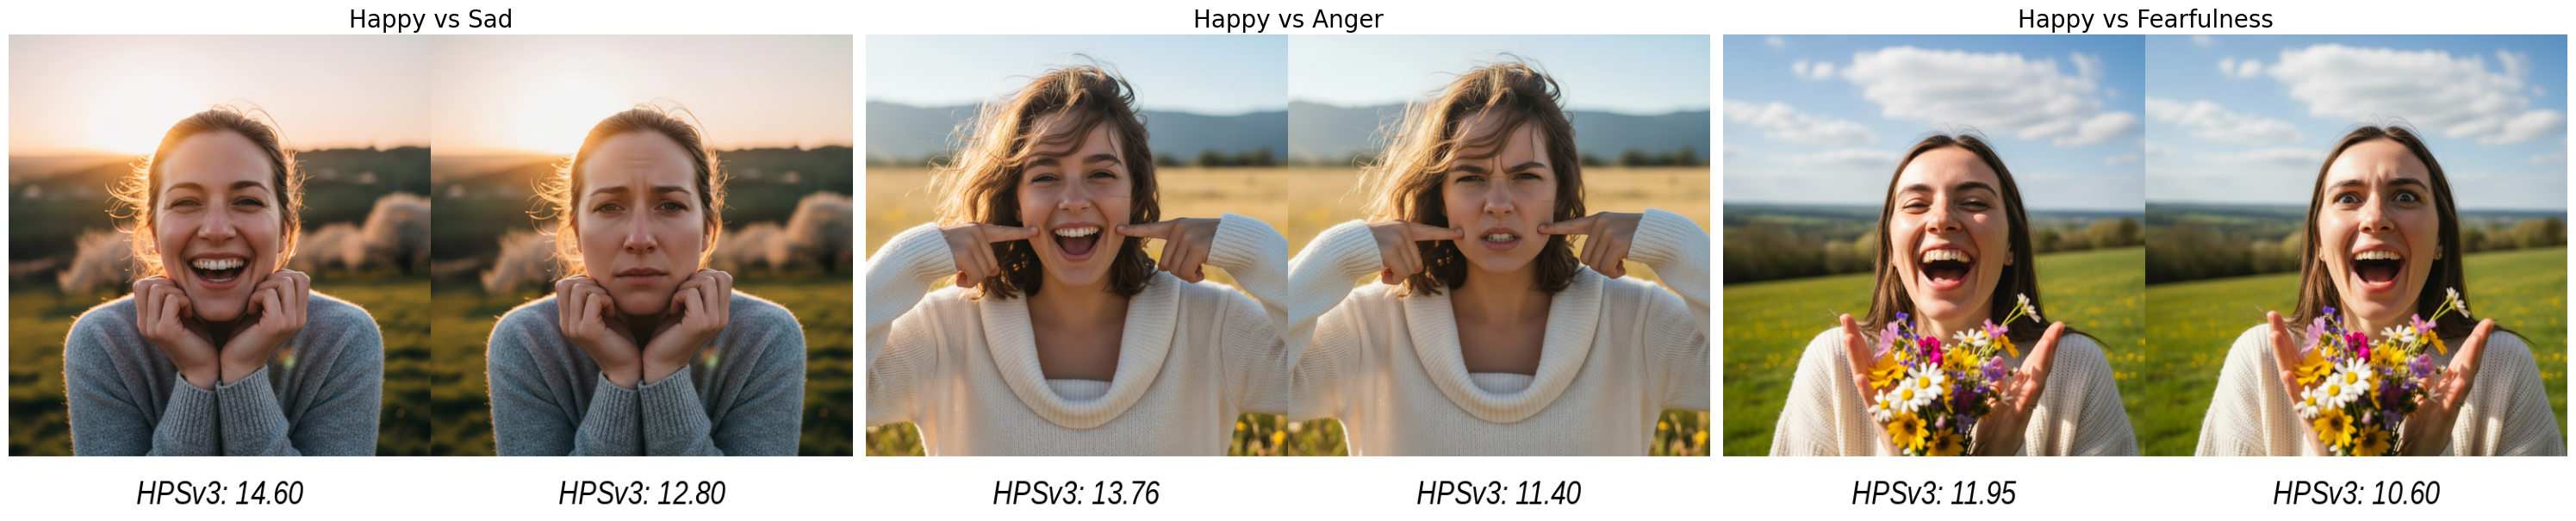
\includegraphics[width=\linewidth]{sec/imgs/emotion.png}
 \caption{Emotion Bias Rating by HPSv3: all images were rated using prompts describing negative emotions, yet HPSv3 consistently assigned higher scores to the positive emotion images.}
 \label{fig:emotion_bias}
 \vspace{-10pt}
\end{figure}

\label{sec:emotion}
As discussed in the Introduction, negative emotions—similar to wide-spectrum aesthetics—play a key role in art expression and real life. Although we examined emotion as one dimension of wide-spectrum aesthetics from VisionReward, we also conducted a more controlled test. 

To minimize noise and bias from unrelated elements, we first generated an image expressing happiness using Nano Banana, then applied image-to-image editing with Nano Banana to create versions expressing negative emotions: sadness, anger, and fearfulness. Everything besides the emotion was aimed to be unchanged. Examples and their corresponding scores are shown in Fig~\ref{fig:emotion_bias} in the Appendix. 

We also evaluated this as a classification task. If the reward model selected the image matching the negative emotion, it was considered correct. Quantitative results are reported in Table~\ref{tab:emotion}. The result shows that reward models are very opinionated against negative emotions, even when the prompt contains negative emotions.

Additionally, we tested how an aesthetics-aligned model will generate when the user asks for a negative emotion face on the Flux family models. We found that if the prompt describes neutral elements and only mentions the emotion in a single place, a highly-aligned model (DanceFlux) usually fails to follow the prompt, unlike an unaligned model. They usually generated neutral or even positive emotions when given prompts containing negative emotions. However, when prompted to generate happy faces, DanceFlux can generate them. This confirmed our concerns about toxic positivity in image generation models, and it is the opposite finding compared to earlier research, which shows models tend to generate negative emotion content \cite{mehta_emotional_2024}. 


\begin{table}[t]
 \centering
 \caption{Negative emotion classification accuracy across different models.}
 \scalebox{1.0}{
 \begin{tabular}{llll}
 \toprule
 {Model} & {Anger} & {Fearfulness} & {Sadness} \\
 \midrule
 BLIP & \textbf{0.960} & \textbf{0.790} & \textbf{0.950} \\
 HPSv2 & 0.700 & 0.640 & 0.880 \\
 HPSv3 & 0.190 & 0.320 & 0.440 \\
 ImageReward & 0.550 & 0.490 & 0.770 \\
 \bottomrule
 \end{tabular}}
 \label{tab:emotion}
 \vspace{-0.1in}
\end{table}


\begin{table}[t]
 \centering
 \caption{Emotion generation scores for each model. The scores show how well the model generates the specific emotion, measured by BLIP.}
 \scalebox{1.0}{
 \begin{tabular}{lrrrr}
 \toprule
 & Angry & Fearful & Happy & Sad \\
 \midrule
 DanceFlux & 0.27 & 0.33 & 0.61 & 0.36 \\
 Flux Dev & 0.51 & 0.50 & 0.50 & 0.48 \\
 Flux Krea & 0.65 & 0.45 & 0.60 & 0.55 \\
 PrefFlux & 0.49 & 0.63 & 0.54 & 0.50 \\
 Nano Banana & 0.84 & 0.80 & 0.60 & 0.70 \\
 SD3.5-Large & 0.89 & 0.49 & 0.62 & 0.50 \\
 \bottomrule
 \end{tabular}}
 \label{tab:emotion_gen}
 \vskip -0.2pt
\end{table}

To test the generative model's ability to capture the full spectrum of emotions, we performed emotion generation tests on the Flux family. SDXL often failed to render a person facing the camera, and Stable Diffusion 3.5 sometimes produced failed faces, so we excluded those families and added Stable Diffusion 3.5 Large (guidance scale 4) as an unaligned baseline to rule out that smaller models cannot understand emotions. Nano Banana was included as an external baseline. All models besides Nano Banana share the same seed. We created 30 emotionally neutral prompts with a \texttt{[emotion]} placeholder and instantiated each with happy, sad, fearfulness, or anger, yielding 120 prompts. The resulting image was cropped with the open-vocabulary detector LLMDet \cite{fu_llmdet_2025} to the human face and scored by BLIP with the prompt \texttt{The face shows [emotion] expression}. For each model and emotion, we recorded the target-emotion score averaged across prompts (Table~\ref{tab:emotion_gen}). DanceFlux, strongly aesthetics-aligned, consistently executed happy prompts but failed on most negative emotions, whereas Flux Krea and Stable Diffusion 3.5 Large followed negative-emotion prompts much better. Flux Dev and PrefFlux fell between these extremes, suggesting that PrefFlux's alignment via UniGenBench preserved prompt following by rewarding competence on complex instructions. This finding differs from earlier research where image generation models tend to generate negative emotion content \cite{mehta_emotional_2024}. We expressed our concerns here, for overly optimistic and positive emotions could be problematic because they create an environment of toxic positivity and an ideological bias that positive emotion is always good and appropriate. It is also a symptom of optimization toward likeability rather than truth, both to the real world and the user's prompt.


\subsection{Validation on Real Images}


\begin{figure*}[!t]
    \centering
    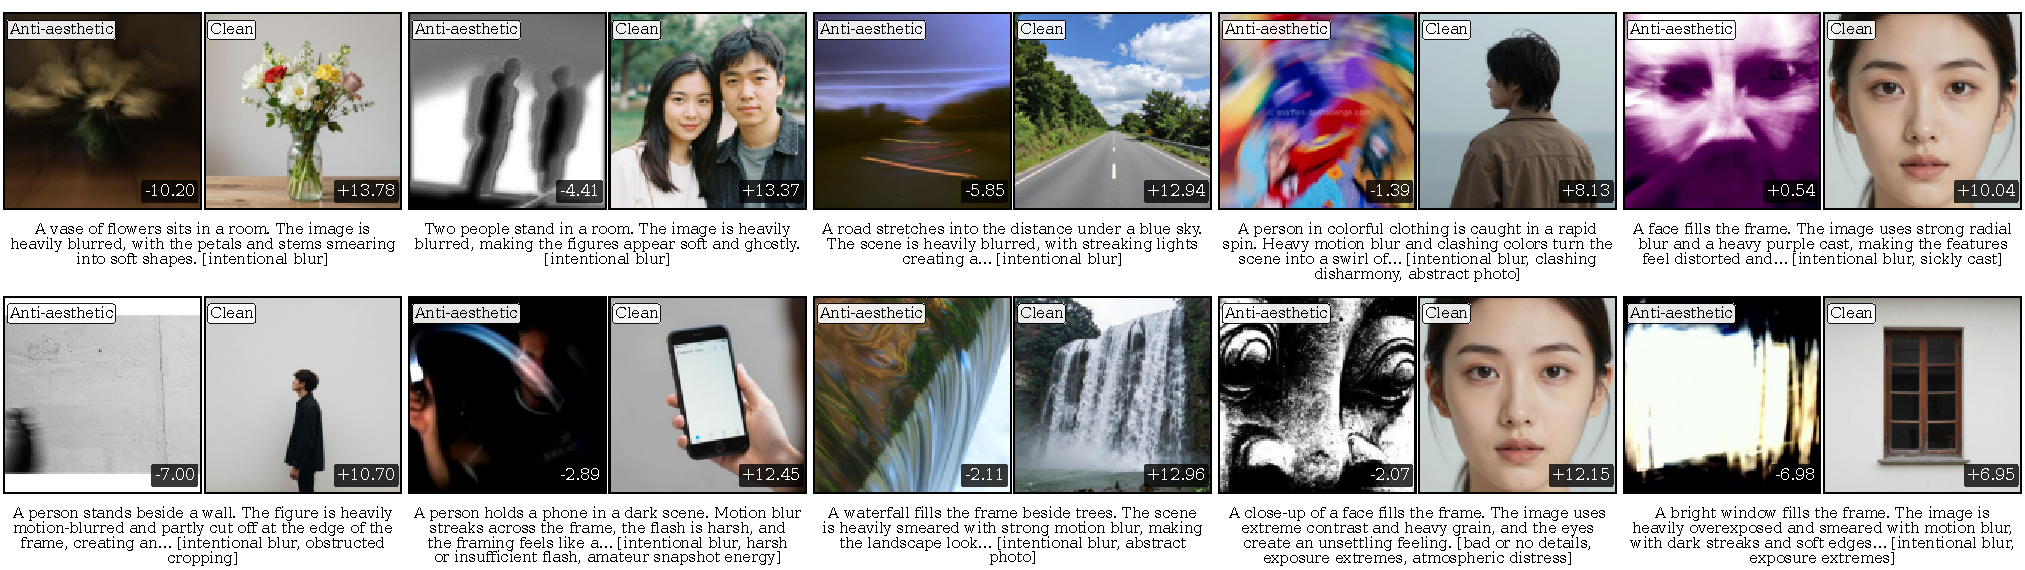
\includegraphics[width=\linewidth]{sec/imgs/figure_reward_comparison.pdf}
    \caption{HPSv3 assigns significantly lower scores to professionally anti-aesthetic images than to clean but thematically incorrect images, even when the prompt explicitly requests anti-aesthetic elements, indicating a bias toward a universal standard of beauty.}
    \label{fig:diff}
\end{figure*}
We also evaluated reward models on real photography. Real images are not out-of-distribution for HPSv3, since its training data includes real images as an upper bound.

To source deliberately anti-aesthetic photographs, we drew on the AVA dataset \cite{murray_ava_2012}, which provides explicit category labels (e.g., motion blur, image grain). Because AVA images come from professional photography platforms, anti-aesthetic traits can be treated as intentional stylistic choices rather than accidental defects. We targeted five classes: clarity, color, lighting, composition, emotions, and subjects, and used an agentic workflow with an LLM to curate the dataset.

The agent's primary tool is an image-text retrieval model built on Gemini Embedding 2 Preview. The LLM (Claude Opus 4.7) decomposes each class into sub-classes and iteratively refines retrieval prompts, yielding 6.27K distinct images. GPT-5.4-Mini then judges whether each image is genuinely anti-aesthetic and writes two captions per image: an anti-aesthetic prompt (visual content + retrieved style) and a ``clean'' prompt (content only). After filtering, 2,928 images remain.

Z-Image Turbo \cite{team_z-image_2025} generates a clean image from each clean prompt. We compare the reward model scores on the original anti-aesthetic photograph and the generated clean image, both conditioned on the anti-aesthetic prompt. If the reward model respects user intent, the original photograph should score higher since the clean image was generated from a different prompt that omits the requested style. We hypothesize the opposite. Indeed, HPSv3 rates the clean image 5.90 points higher on average; the gap is largest for Analog Degradation (13.2) and around 8 for Intentional Blur and Exposure Extremes (full table on our GitHub repo; HPSv3's range is roughly 0-15, technically unbounded). This confirms that HPSv3 strongly favors clean, polished images over purposefully anti-aesthetic ones. Figure~\ref{fig:diff} shows several largest-difference examples to illustrate that these images are not simply ``ugly'' but genuine anti-aesthetic artwork that HPSv3 cannot appreciate.

The gap here is much larger than for AI-generated images, likely because AI images, even when anti-aesthetic, retain a ``polished AI look''. When we restrict the comparison to GPT-Image or Nano Banana outputs (which lack this polished look), the gap remains large.

We extended this analysis to real artworks. Using $\sim$10K paintings from the LAPIS dataset \cite{maerten_lapis_2025} captioned with \texttt{Qwen/Qwen3-VL-30B-A3B-Instruct}, we compared their HPSv3 scores against the official HPSv3 leaderboard. Real art averages a raw HPSv3 of 5.86, placing 10/12 on the Aug 2025 leaderboard, just above Hunyuan-DiT and below most modern image generators. Many individual works drop well into negative territory despite being clearly composed paintings (Figure~\ref{fig:real_arts}). To rule out that reward models cannot understand these images, we computed BLIP on the same image-caption pairs and got 0.996; shuffling captions and images dropped this to 0.086. Reward models could thus understand the content but choose to penalize works that deviate from mainstream taste.

\begin{figure}[h]
    \centering
    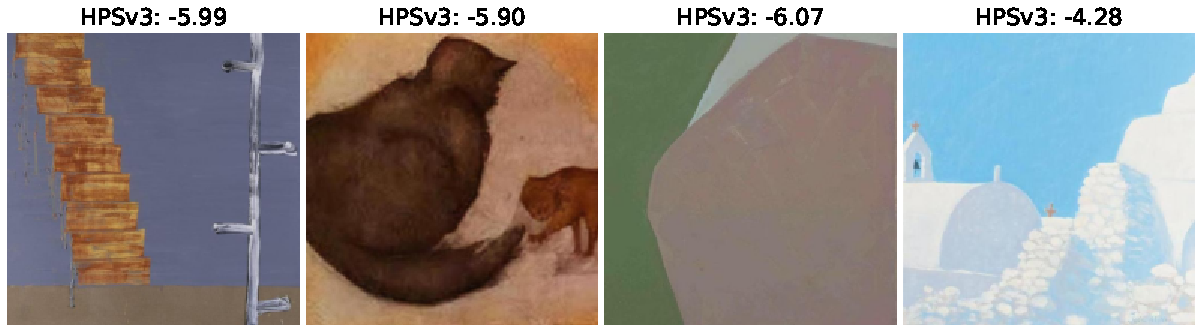
\includegraphics[width=\linewidth]{sec/imgs/real_arts.pdf}
    \vspace{-15pt}
    \caption{Real paintings from the LAPIS dataset \cite{maerten_lapis_2025} that HPSv3 scores well below typical AI-generated images. Both representational works and abstract compositions are penalized, regardless of artistic intent.}
    \label{fig:real_arts}
    \vspace{-10pt}
\end{figure}

\section{Alternative Positions and Rebuttal}


\textbf{The ``wide-spectrum aesthetics'' represents technical flaws rather than artistic subversion, and a default experience pleasing the majority is a pragmatic design choice.} Among our dimensions, only ``clarity'' might be considered a technical flaw; the others (e.g., emotion, realism, brightness) are stylistic or artistic choices. Even low clarity is often deliberately used to convey emotion, motion, or narrative \cite{stacey_hill_embracing_nodate}. Constraining these dimensions limits user expression and control. 

On majority preferences, we follow \citet{guo_position_2025} in arguing that minority experiences should not be sacrificed to please the majority. Doing so marginalizes users with niche needs and enforces majoritarianism. Many users choose AI precisely because it combines low barriers to use with near-unlimited control, similar to professional tools (e.g., Photoshop) but more accessible. They can request impossible scenes and freely adjust any attribute. More importantly, as discussed in Section~\ref{sec:reversed_alignment}, the reversed alignment not only creates inconvenience for minorities but also actively pushes them to align with and assimilate into the majority. When users' explicit prompts are overridden by a sanitized output presented as the ``correct'' image, the system does not merely fail to follow instructions; it implicitly communicates that the user's intended aesthetic is wrong, reinforcing the assimilation effect described above.


As in \citet{guo_position_2025}, which calls for balance rather than overcaution in health queries, supporting wide-spectrum aesthetics does not reduce the quality of conventionally ``good'' images. It enlarges the expressive range so users can obtain diverse aesthetics while still accessing high-quality traditional outputs. Models like Nano Banana and GPT-Image already do this, excelling at both traditional, high-quality images and wide-spectrum aesthetics, as shown in the Appendix.


\section{Conclusion}
This work demonstrates that aesthetic alignment in image generation systematically suppresses legitimate creative expression. Reward models penalize images faithful to wide-spectrum aesthetics prompts, generation models override explicit user instructions in favor of conventionally beautiful outputs, and historically significant artworks receive scores far below AI-generated images. Optimization toward an imaginary average, which we named \emph{reversed alignment}, is not merely making part of the users inconvenienced; it is actively erasing the concrete intentions of actual individuals, functioning as aesthetic authoritarianism that narrows admissible expression and removes the capacity to dissent from imposed norms.


